\section{The Spectrum of Sound}

El so és la vibració d'un cos que es transmet per l'aire i es percep per la nostra oïda. Si mous la mà amunt i avall una vegada per segon, diem que la ma vibra a la freqüència d'1 Hertz (Hz). Si la mous amunt i avall dues vegades per segon, la freqüència és de 2 Hz. Si ho poguessis fer 20 vegades per segon (20 Hz), segurament les teves orelles podrien començar a notar la vibració transmesa a través de l'aire. Segurament no pots fer-ho amb la mà, però pots fer servir la corda d'una guitarra, la membrana d'un timbal, l'aire dins d'una flauta, les teves cordes vocals, el cos d'una campana... Normalment una persona pot sentir vibracions amb una freqüència d'entre 20 i 20 000 Hz. Com més alta és la freqüència, més alt és el to del so que sentim.

De totes maneres, si els cossos que fas vibrar són una corda de guitarra o una flauta notaràs que els sons que percebràs són molt diferents entre ells. Això es deu al fet que gairebé mai sentim una freqüència ''pura'', qualsevol so natural és un conjunt de vibracions a diferents freqüències amb diverses intensitats. Una corda de guitarra afinada al La central vibrarà a 440 Hz. Aquesta és l'anomenada freqüència fonamental, però la corda inevitablement també vibrarà a 880 Hz (el doble), a 1320 Hz (el triple), i a la resta de freqüències múltiples, que són les anomenades freqüències harmòniques, però cada vegada amb menor intensitat. Una flauta també vibrarà a aquestes freqüències, però amb un conjunt d'intensitats diferent. És precisament aquesta variació en la intensitat de les freqüències harmòniques la que fa que la nostra oïda distingeixi el so de la guitarra del d'una flauta. El conjunt de freqüències i les seves intensitats s'anomena l'espectre del so, i defineix el que anomenem el timbre al món de la música.

\begin{wrapfigure}[15]{l}{0.35\textwidth}
\centering
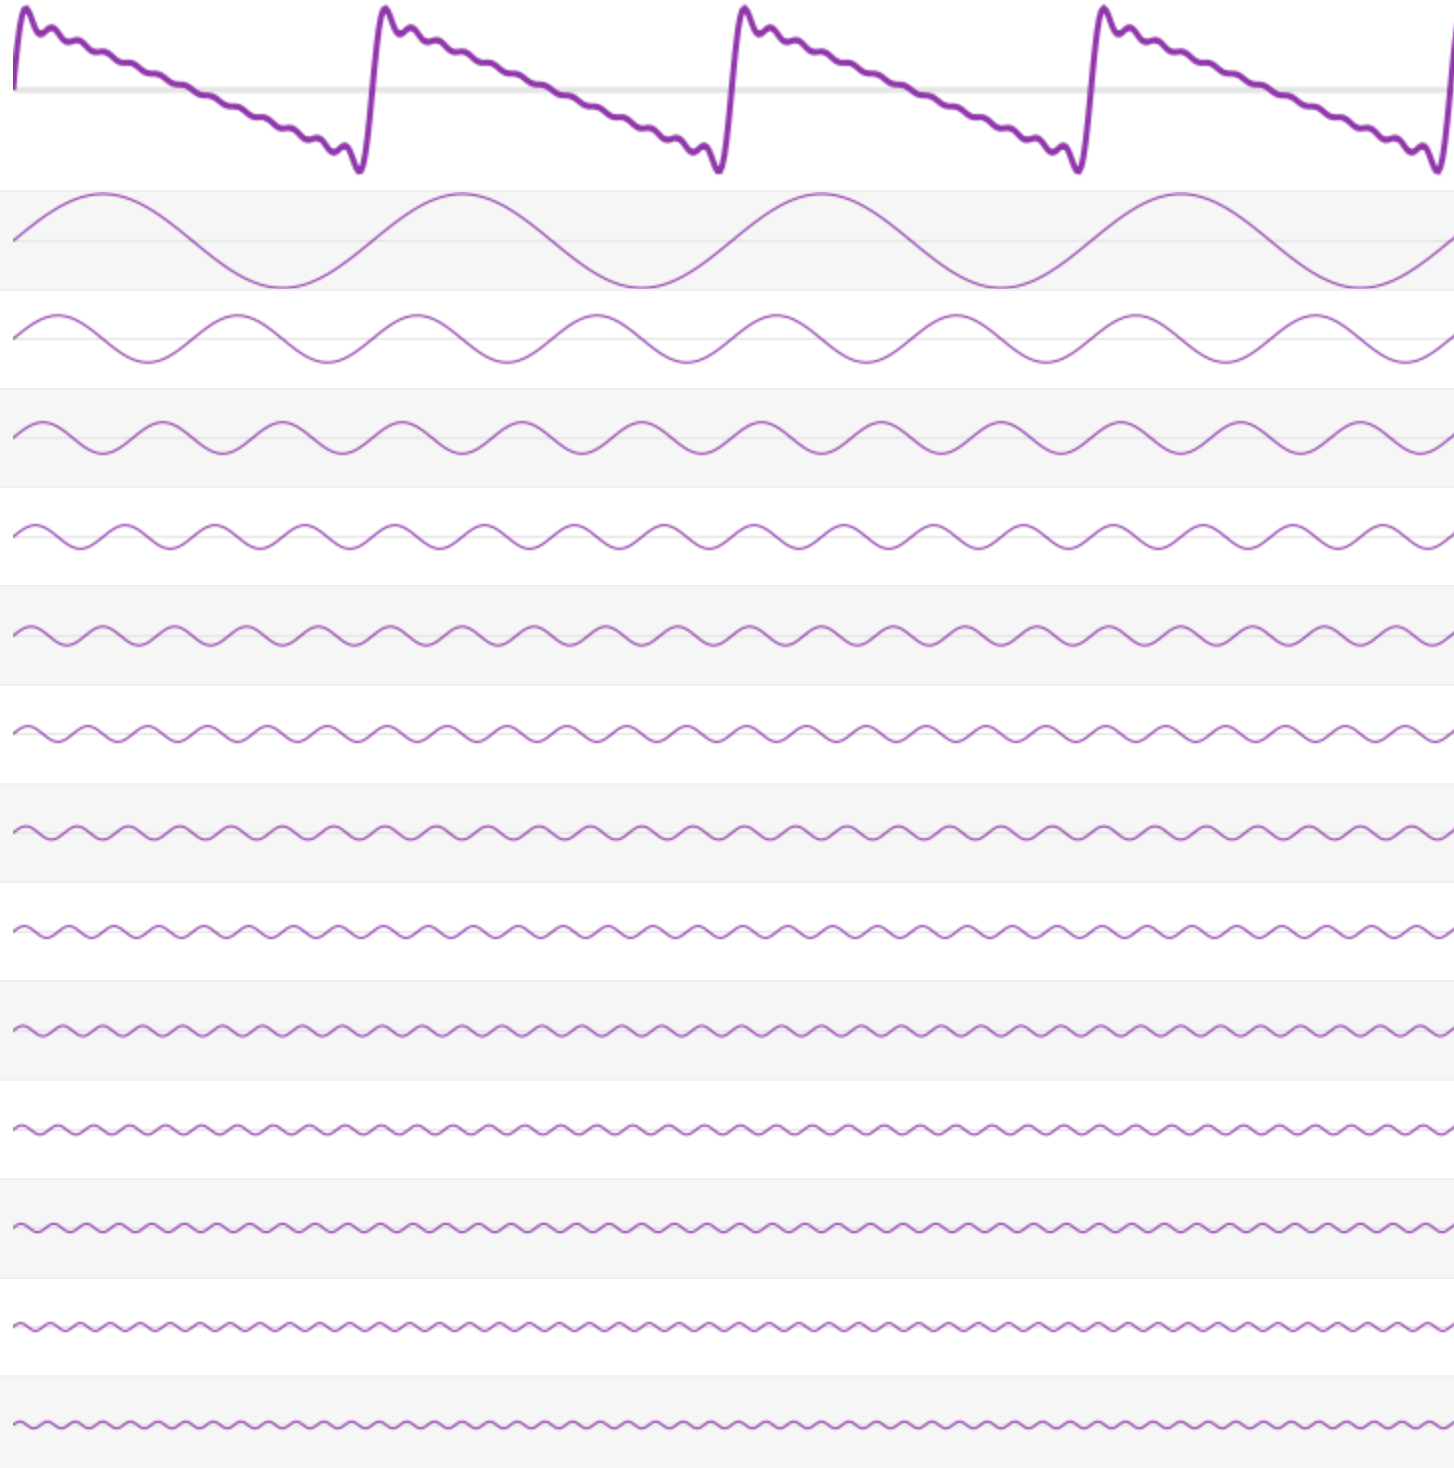
\includegraphics[width=0.35\textwidth]{SpectrumOfSound_1}
\caption*{Una ona de dent de serra vista com la suma d'ones sinusoidals.}
\end{wrapfigure}

I què seria un so ``pur'', només una freqüència sense cap mena de ``contaminació'' d'altres? Matemàticament, podem descriure aquest so com una ona sinusoidal. És el so que faria una molla perfectament elàstica que pogués vibrar sense perdre energia. No podem construir una molla amb aquestes característiques, però podem fer que la membrana d'un altaveu vibri a aquesta freqüència pura fent servir electrònica. Un resultat tant sorprenent com útil de les matemàtiques és el fet que tota funció periòdica de període $2\pi$ es pot aproximar amb una suma d'una seqüència d'ones sinusoidals, si s'escalen i es desfasen adequadament. Vist en una formula:
$$g(t) \approx A_0 + \sum_{i=1}^N A_i \cdot \sin(i t + \varphi_i).$$


Això implica que sumant les ones sinusoidals adequades podem simular qualsevol so estàtic. L'única informació que necessitem és el conjunt d'intensitats $A_i$ i desfasaments  $\varphi_i$. Això té implicacions molt profundes. Per una banda permet descompondre un senyal complex en un conjunt de senyals molt més simples de forma molt estructurada, fent-lo molt més senzill d'entendre i analitzar. A un nivell més abstracte també connecta diferents dominis: el domini temporal on els senyals es descriuen amb valors (com la pressió de l'aire) que varien amb el temps i el domini de la freqüència on els senyals es componen d'altres més simples. Segons la situació, pot ser molt útil afrontar un problema des d'un domini o un altre.

Les seves aplicacions són d'un abast molt ampli i cobreixen àrees molt diverses a més a més del so i la música, com ara la tecnologia de la comunicació, teoria quàntica, teoria de codis, estadística, disseny de circuits elèctrics i una llarga llista d'altres temes.

A la primera pantalla del mòdul, pots provar de generar una ona amb l'addició de freqüències harmòniques. Fes servir només una freqüència (sinusoidal) per sentir un so ``matemàticament pur''. Per sentir diferents timbres, ajusta la intensitat de cada freqüència harmònica, o clica sobre les ones quadrades o de dent de serra.

Heurísticament, un instrument de corda té harmònics més intensos i, en canvi, un instrument de vent els té menys intensos. Però, de totes maneres, estem molt lluny d'un sintetitzador complet. Per simular un instrument real, hem de tenir en consideració que el so no és estàtic ni etern, comença a un punt, augmenta d'intensitat i, per acabar, decau i s'esvaeix. És a dir, les freqüències i les seves intensitats canvien amb el temps. Els instruments com les campanes, xilòfons i molts d'altres de percussió no tenen un espectre format per múltiples de la fonamental, sinó per la forma geomètrica del cos que vibra. Per aquests motius, és força complicat sintetitzar un instrument real.

De totes maneres, hi ha una eina matemàtica extraordinària que ens permet invertir el procés. En comptes de sumar freqüències per obtenir un senyal compost, la transformada de Fourier és el procés que permet descompondre un senyal arbitrari (gravat amb un micròfon, per exemple) en les seves parts fonamentals: les freqüències i les seves intensitats que et caldrien per generar el senyal a partir de freqüències pures.

Imagina que $g(t)$ és un senyal representat com una funció que per cada instant de temps t retorna la intensitat del so (aquesta intensitat pot ser la pressió de l'aire o el voltatge al cable del micròfon). La transformada de Fourier del senyal $g(t)$ és una nova funció $\hat g(t)$ que, per cada freqüència $f$, retorna la intensitat que hauria de tenir l'ona sinusoidal d'aquella freqüència per sintetitzar el senyal $g(t)$. La transformada de Fourier es pot aconseguir amb aquesta formula:
$$\hat g(f) = \int_{-\infty}^{\infty} g(t)\ e^{2\pi i f t } \ dt$$

\begin{wrapfigure}[13]{r}{0.45\textwidth}
\centering
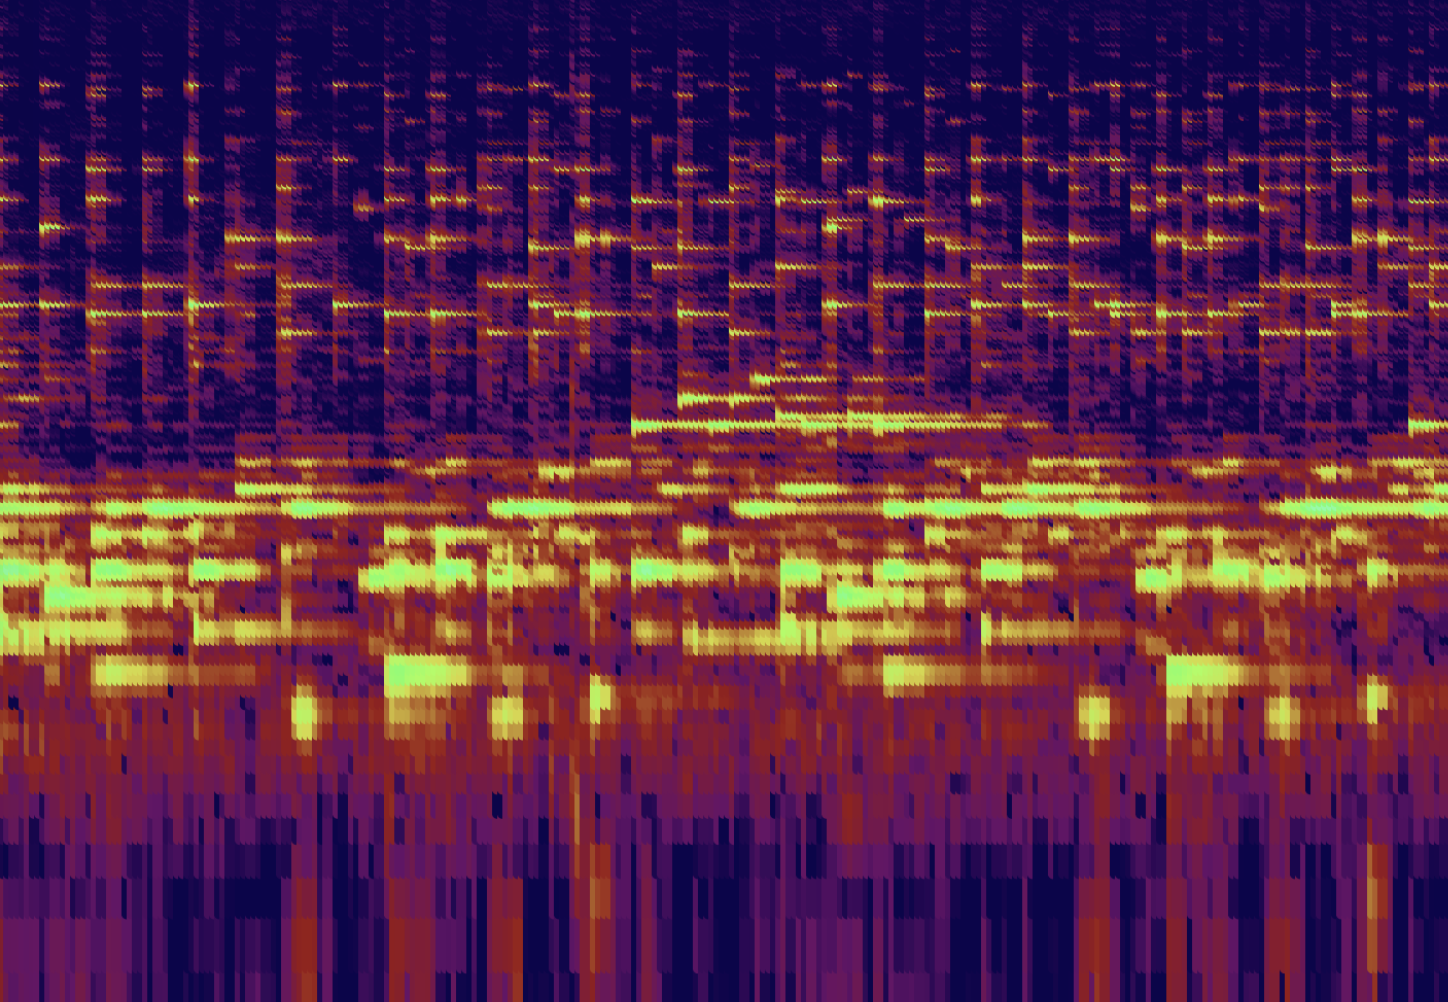
\includegraphics[width=0.45\textwidth]{SpectrumOfSound_2}
\caption*{Sonograma de part del Cànon de Pachelbel.}
\end{wrapfigure}

Fixa't que hi ha valors complexos dins l'integral i, per aquest motiu, la transformada de Fourier és una funció que pot prendre valors complexos. Això és degut a les dues informacions necessàries per sintetitzar un senyal: l'amplitud $A_i$ i els desfasaments $\varphi_i$.

La transformada de Fourier ens dona tant l'amplitud com la fase del senyal, respectivament representats en el mòdul i l'argument del valor complex. Normalment, per fer anàlisis d'àudio només s'utilitza el mòdul per obtenir el gràfic amb els pics a les freqüències més notòries, que ja és suficient per reconstruir el senyal original amb precisió.

Per aplicacions pràctiques, hi ha un algorisme molt útil que s'anomena Fast Fourier Transform (FFT) que substitueix l'abstracta formula matemàtica. Aquest algorisme permet càlculs molt ràpids i possibilita l'anàlisi de senyals en temps real. En l'actualitat moltes maneres de treballar amb la música estan basades en la FFT. És el primer pas en l'extracció d'una partitura a partir de la música tocada. Es pot fer servir, per exemple, per fer la transcripció automàtica d'un solo de Jazz. Per altra banda també és la base de la modificació de la música. La correcció tonal (auto-tune) que tant es veu a la música pop de l'actualitat es pot descriure bàsicament com un procés d'``anàlisi - correcció - síntesis''. Altres efectes com fer parlar un instrument amb veu humana també utilitzen l'anàlisis de l'espectre involucrat. També els serveis de reconeixement automàtic de cançons com ara el Shazam depenen de l'empremta d'una peça representada pel seu sonograma.

La segona pantalla del mòdul mostra un analitzador d'espectre connectat a un micròfon. A l'esquerra hi ha l'espectre, que es pot veure com una anàlisi instantània de freqüències (transformada de Fourier) del senyal captat. A la dreta, l'espectre deixa espai per visualitzar l'històric del senyal d'entrada, és a dir, el seu sonograma.

\begin{figure}[h]
\centering
\begin{subfigure}{0.45\textwidth}
\centering
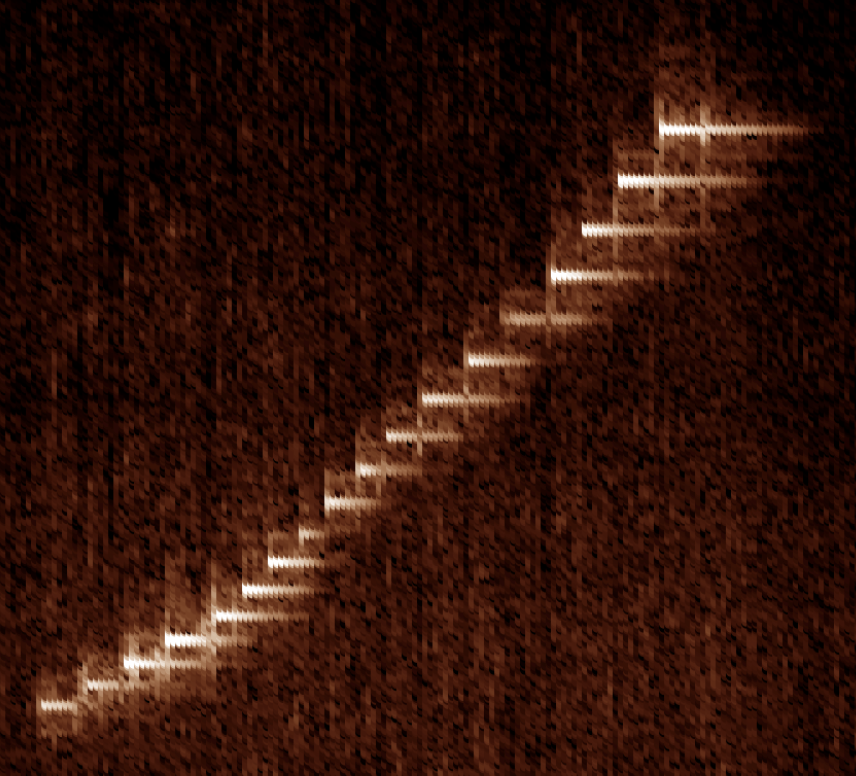
\includegraphics[height=3cm]{SpectrumOfSound_7}
\subcaption*{Chromatic scale linear.}
\end{subfigure}
\begin{subfigure}{0.45\textwidth}
\centering
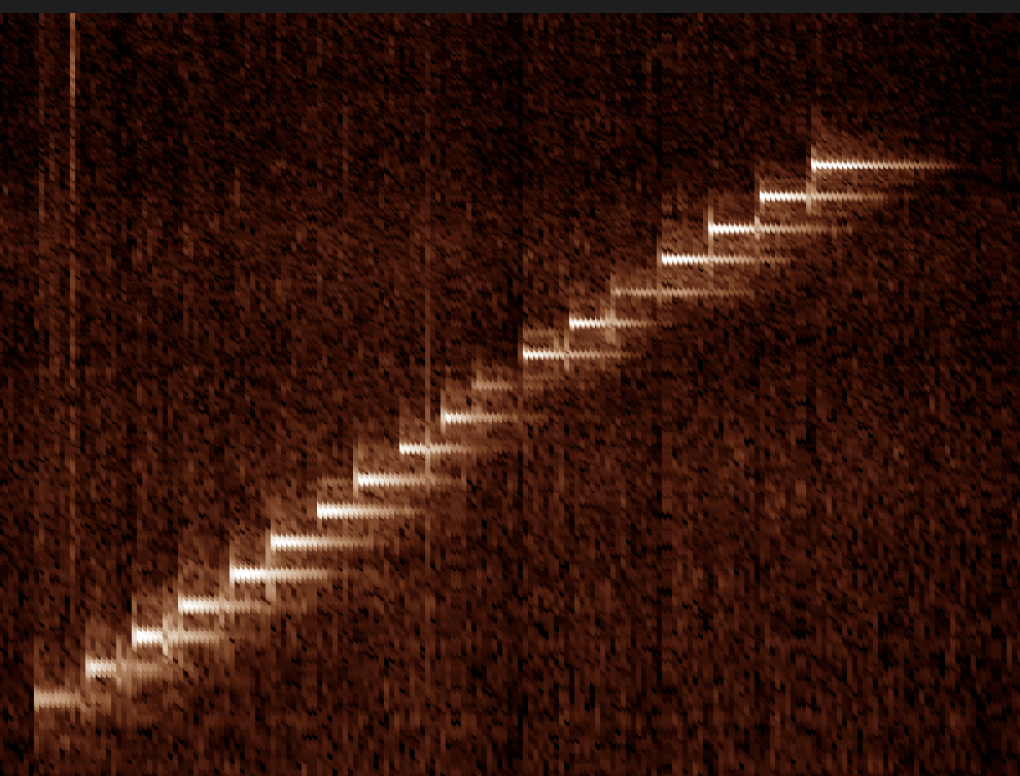
\includegraphics[height=3cm]{SpectrumOfSound_8}
\subcaption*{Chromatic scale logarithmic.}
\end{subfigure}
\end{figure}

L'escala lineal és més útil per sons i matisos (freqüències $f$, $2f$, $3f$, $4f$, $5f$, ...), mentre que l'escala logarítmica resulta més pràctica per veure els tons musicals (freqüències $f$, $af$, $a^2 f$, $a^2 f$, $a^2 f$, ...). Pots fer servir el micròfon per analitzar la teva veu o els instruments disponibles. Canta alguna cosa, fes sorolls, parla, o posa el micròfon prop de l'altaveu i analitza el so que produeix. Prova d'identificar freqüències, les seves intensitats, quan apareixen i quan desapareixen.

\begin{figure}[h]
\centering
\begin{subfigure}{0.45\textwidth}
\centering
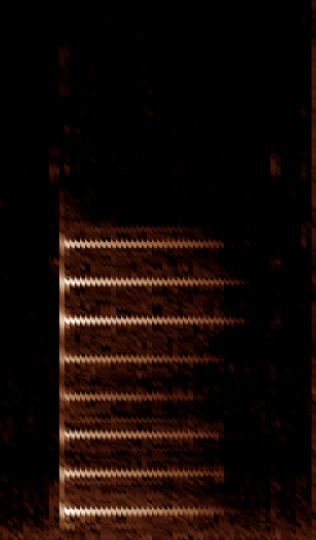
\includegraphics[height=3cm]{SpectrumOfSound_5}
\caption*{Overtones linear.}
\end{subfigure}
\begin{subfigure}{0.45\textwidth}
\centering
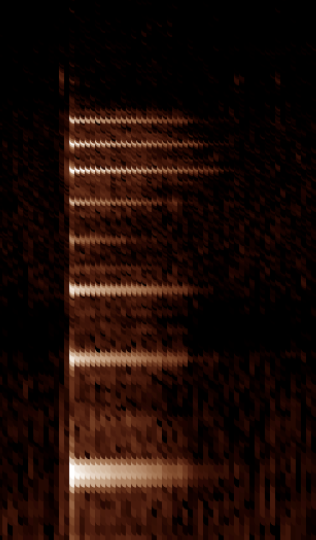
\includegraphics[height=3cm]{SpectrumOfSound_6}
\caption*{Overtones logarithmic.}
\end{subfigure}
\end{figure}


\begin{sectcredits}

\item[Autors del mòdul:]\strut \\
Sintetitzador: Tero Parviainen, Eric Londaits (IMAGINARY). \\
Analitzador: Jürgen Richter-Gebert (TU Munich). \\

\item[Text:] Daniel Ramos (IMAGINARY).

\end{sectcredits}
